\question{Газовые лазеры. Гелий-неоновый лазер.}
\begin{figure}[h]
    \center
    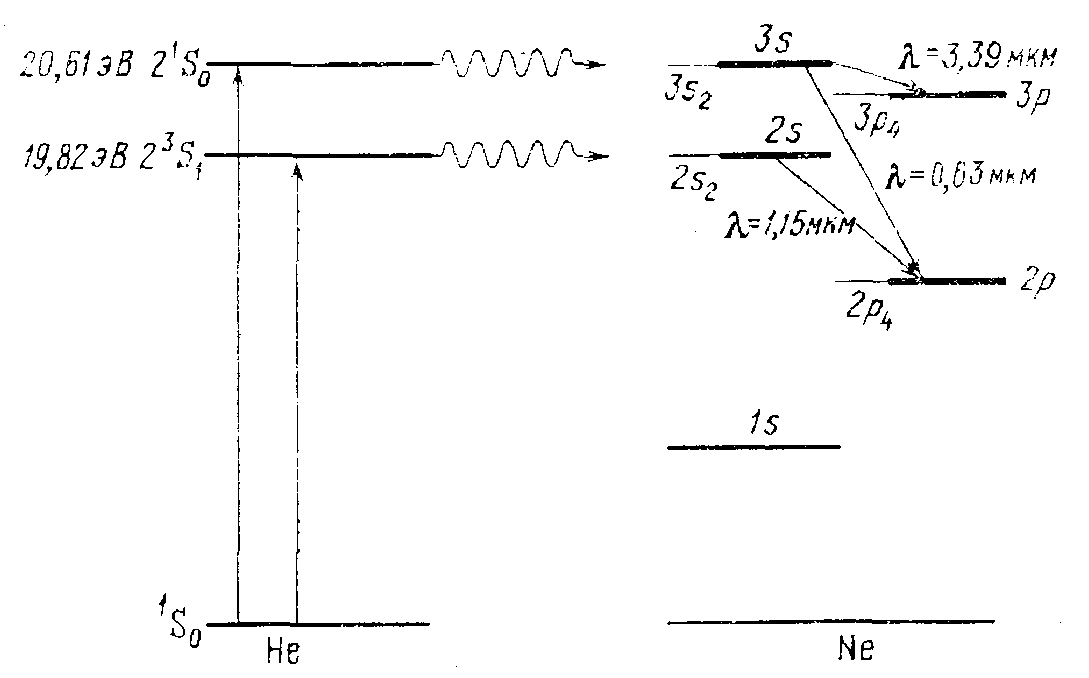
\includegraphics[width=.47\textwidth]{19}
    \caption{Уровни энергии}
\end{figure}
Генерация осуществляется в непрерывном режиме на переходах
\( 3s \rightarrow 2p \) \( (\lambda = 0,63~\text{мкм}) \),
\( 2s \rightarrow 2p \) \( (\lambda = 1,15~\text{мкм}) \) и
\( 3s \rightarrow 3p \) \( (\lambda = 3,39~\text{мкм}) \) нейтральных атомов
неона. Возбуждение верхних лазерных уровней неона происходит при
квазирезонансной передаче энергии возбуждения от гелия неону в процессе
неупругих столкновений.

Метастабильное состояние гелия, столкновительно передающее свою энергию неону, 
возбуждается электронами в плазме тлеющего газового разряда. Для существования 
инверсии в непрерывном режиме необходимо, чтобы нижний лазерный уровень быстро 
опустошался быстрее верхнего. Нижние уровни опустошаются при столкновениях со 
стенками газоразрядной трубки.

Для этого лазера характерна конкуренция линий генерации на \( 0,63 \) и 
\( 3,39 \) мкм, которым соответствует общий стартовый уровень \( 3s \).